\documentclass[9pt,a4paper]{report}
\usepackage{mwe}
\usepackage{listings}
\usepackage{amsmath}
\usepackage{graphicx}
\usepackage{subfig}
\usepackage{float}
\usepackage{xcolor}
\usepackage{multirow}
\usepackage{hyperref}
\usepackage{fancyhdr}
\usepackage{sectsty}
\usepackage[dvipsnames]{xcolor}
\usepackage{soul}
\usepackage[compact]{titlesec}
\usepackage{float}
\usepackage[left=0.5cm,right=0.5cm,top=0.5cm,bottom=0.5cm]{geometry}
\graphicspath{{Full Rectifier circuits/Bridge With Filter}{Full Rectifier circuits/Full Wave Bridge}{Full Rectifier circuits/Bridge With Zener}}

\newcommand*{\nchapter}[1]{%
	\chapter*{#1}%
	\addcontentsline{toc}{chapter}{#1}
	\vspace{-14mm}}
\newcommand*{\nsection}[1]{%
	\section*{#1}%
	\addcontentsline{toc}{section}{#1}}
\newcommand*{\nsubsection}[1]{%
	\subsection*{#1}%
	\addcontentsline{toc}{subsection}{#1}}
\newcommand*{\nsubsubsection}[1]{%
	\subsubsection*{#1}%
	\addcontentsline{toc}{subsubsection}{#1}}

\chaptertitlefont{\large}
\sectionfont{\normalsize}
\fontsize{9}{11}\selectfont
\begin{document}
	\begin{titlepage}
		\centering
		\vspace*{1.5in}
		
\includegraphics[width=0.15\textwidth]{W-Logo_Purple_RGB}\par\vspace{1cm}
		{\LARGE \textsc{University of Washington}\par}
		\vspace{1cm}
		{\Large \textsc{BEE331 Lab 1.2}\par}
		\vspace{1.5cm}
		{\huge\bfseries \par}
		\vspace{2cm}
		{\Large\itshape 2301991\hspace{55pt}1900585\par}
		{\Large\itshape Jason Truong\hspace{31pt}Henry Haight\par}
		\vfill
		supervised by\par
		Prof.~Joseph \textsc{Decuir}
		\date{2024\\ January}
		\vfill
		% Bottom of the page
		{\large \today\par}
		\vspace*{1.5in}
	\end{titlepage}
	
	\nchapter{Full-Wave Bridge Rectifier Circuit}
	\nsection{Design Objective}
	In this lab, we introduce ourselves to two voltage rectifying circuits: The Rectifier and Voltage Clamp. We demonstrated this two two applications across 3 circuits. We characterize its function in $V_{out}$.
	\begingroup
	\renewcommand{\cleardoublepage}{}
	\renewcommand{\clearpage}{}
	\nsection{Circuit Design Outline}
	\endgroup
	[Guidelines do not ask for explanation on design. See Below.]
	\begin{figure}[h!]
		\centering
		\caption{Bridge Rectifier Circuits}
		\subfloat[\centering LTSpice + Rudimentary Schematic Full-Wave Bridge Rectifier]{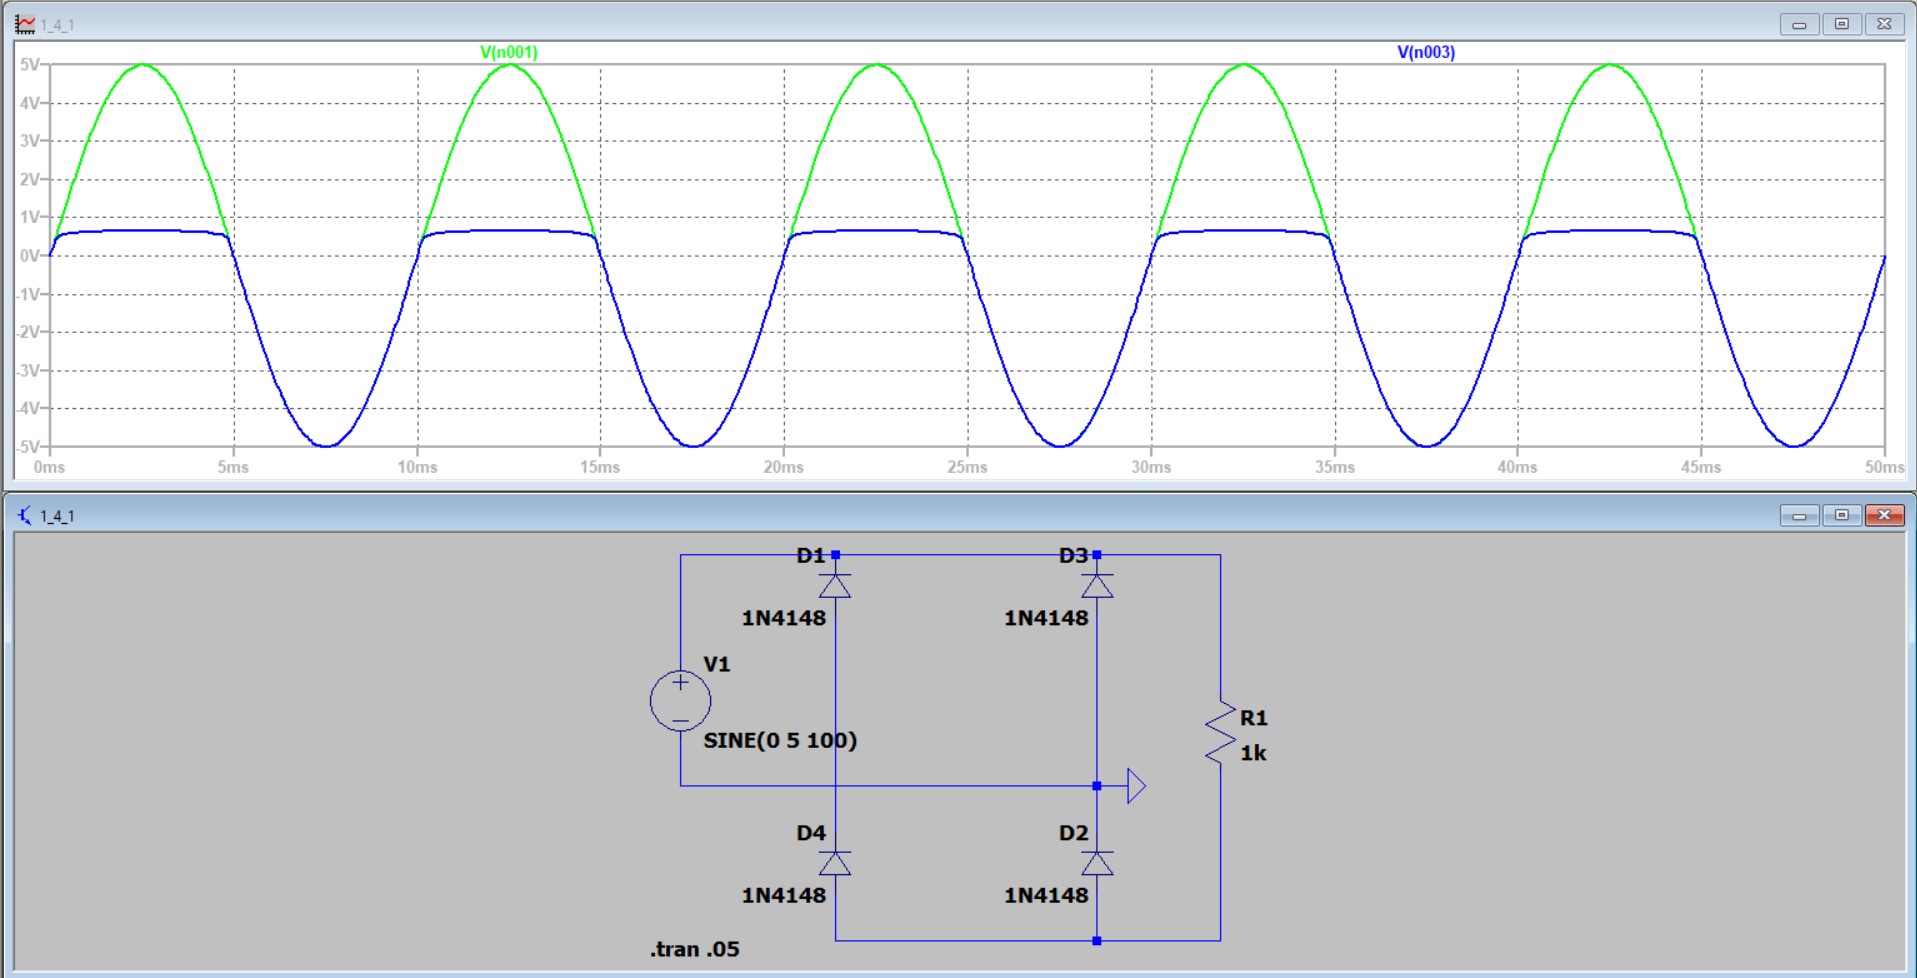
\includegraphics[width=9cm]{Screenshot 2024-07-15 062842}}\hfil
		\subfloat[\centering LTSpice + Rudimentary Schematic Full-Wave Bridge Rectifier with output filter]{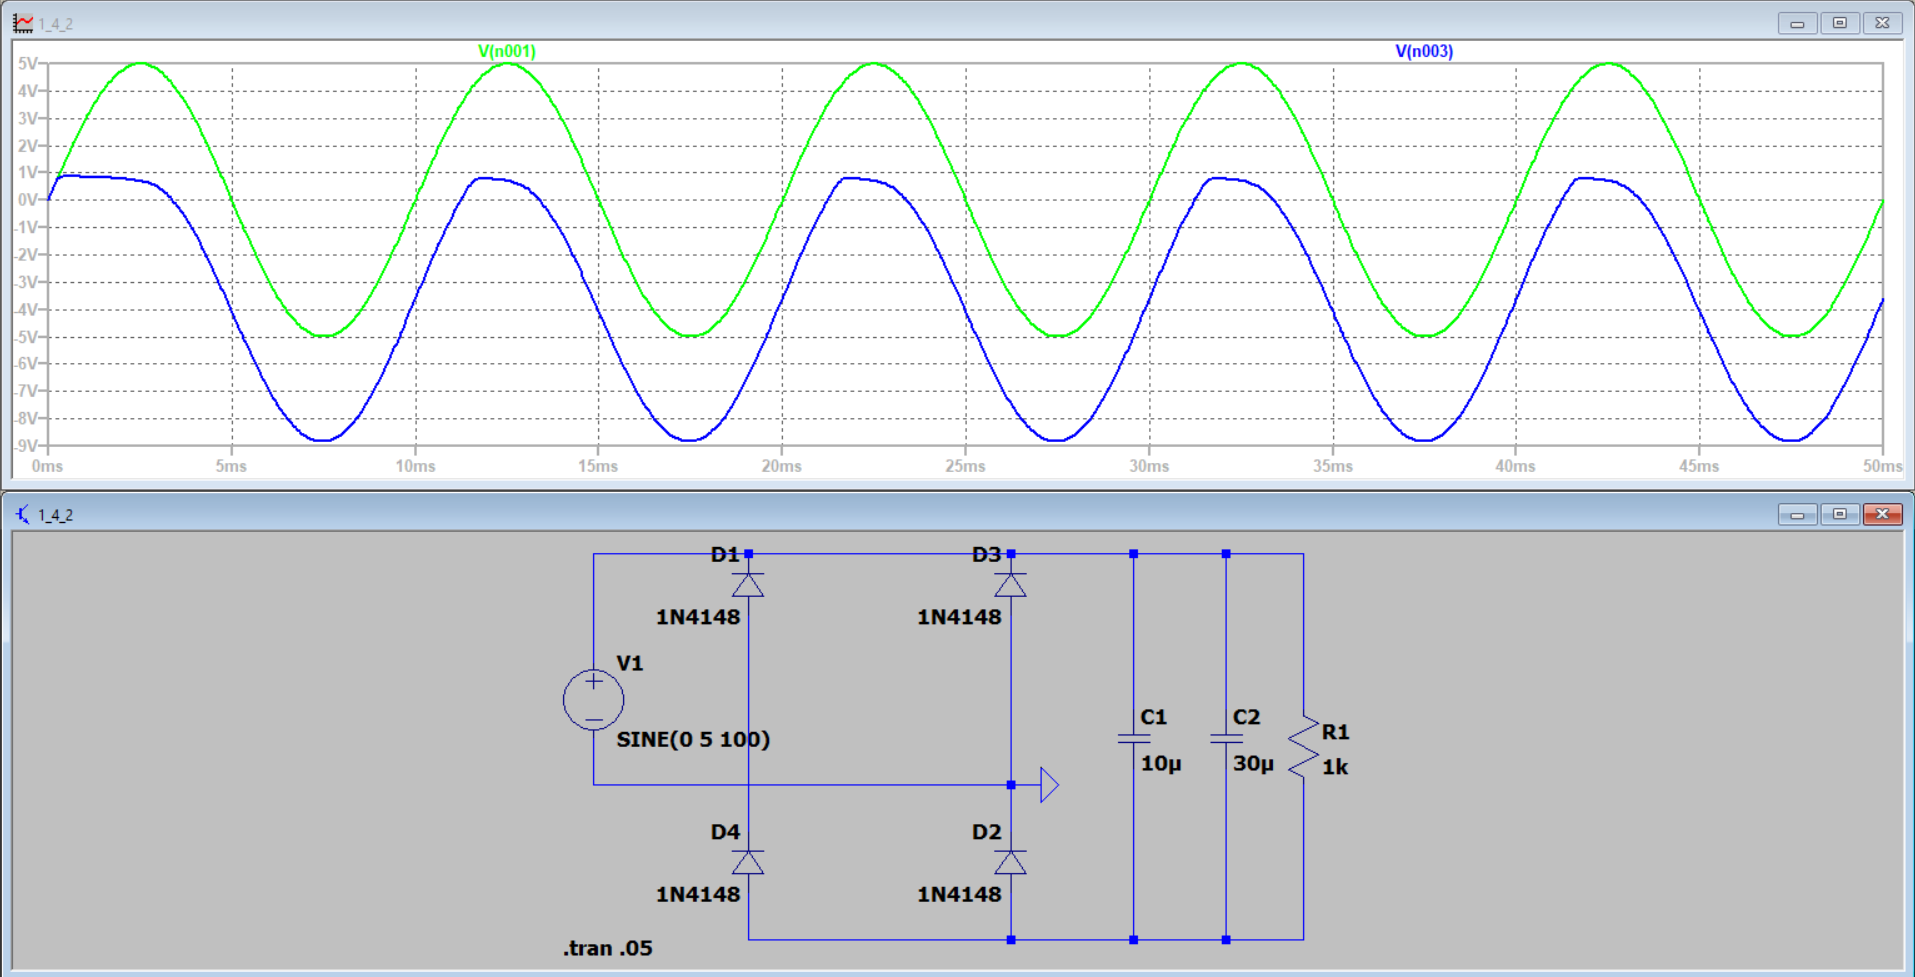
\includegraphics[width=9cm]{Screenshot 2024-07-15 062809}}\hfil
		\subfloat[\centering LTSpice + Rudimentary Schematic Full-Wave Bridge Rectifier with output filter and Zener diode regulator as its output]{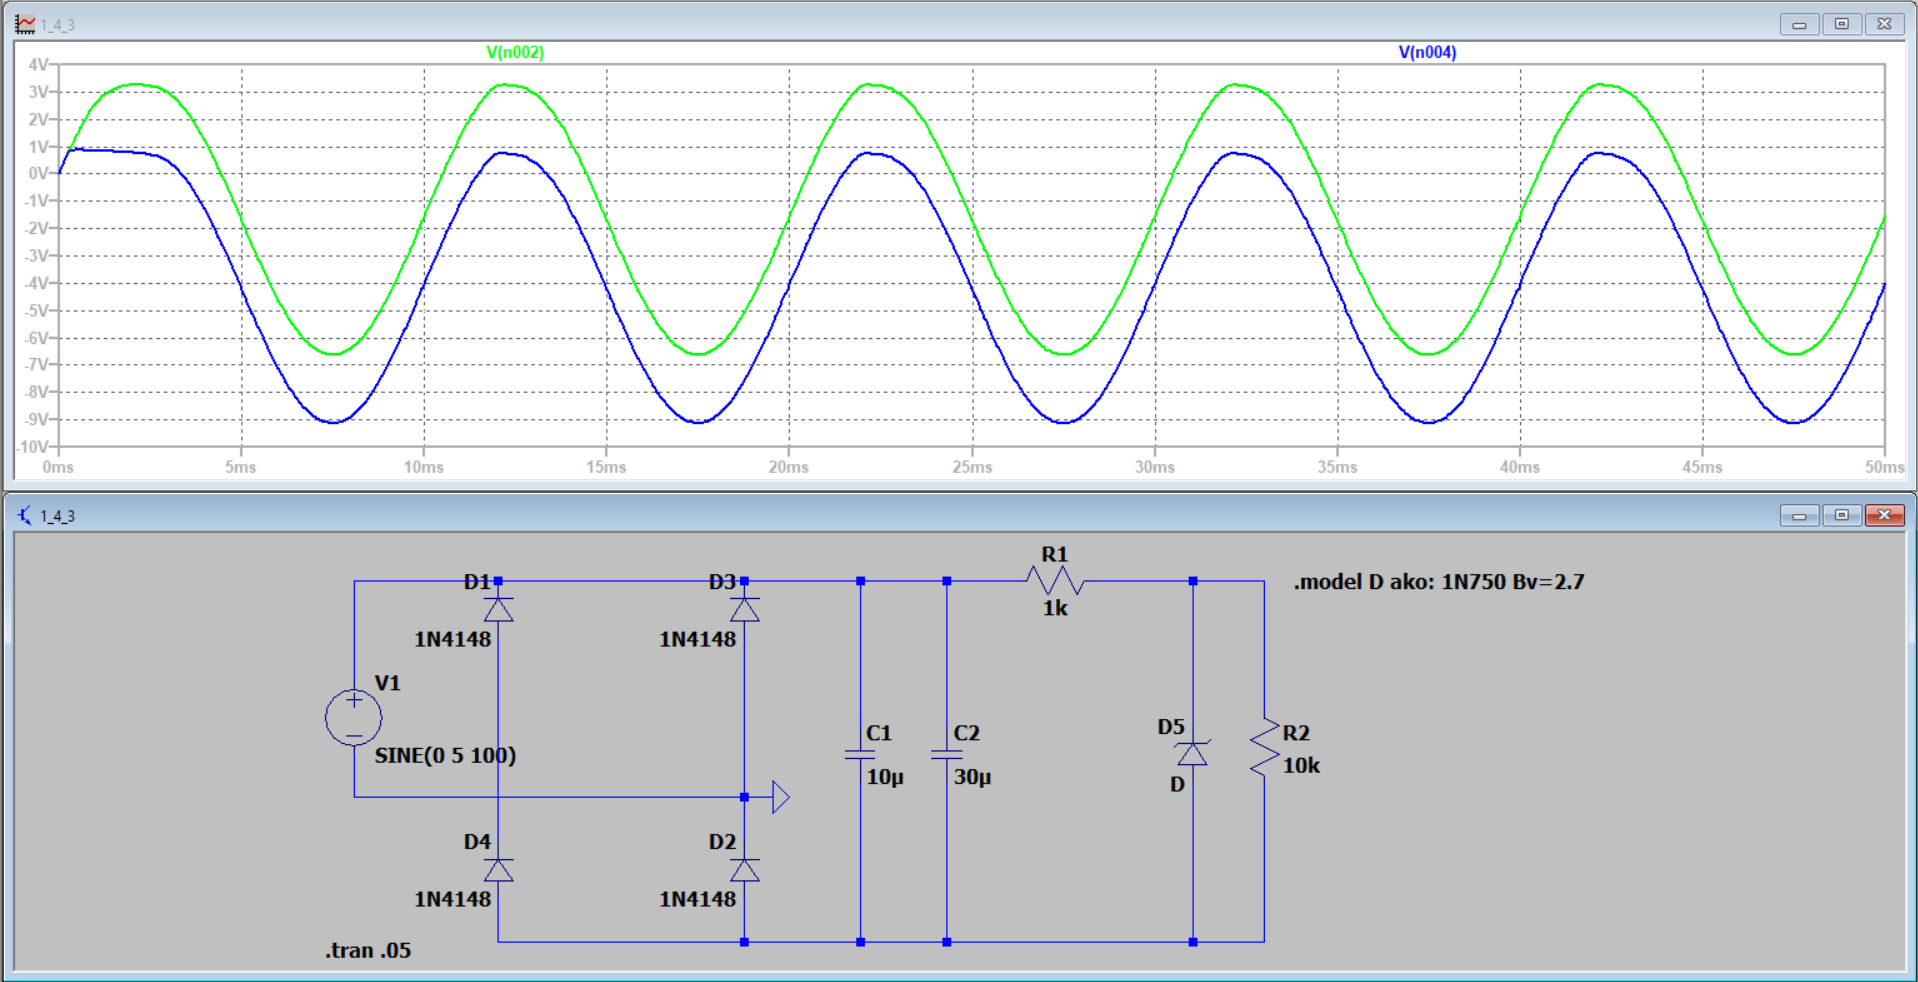
\includegraphics[width=9cm]{Screenshot 2024-07-15 062905}}
	\end{figure}
	
	\begin{figure}[h!]
		\centering
		\caption{Bridge Rectifier Circuits IRL}
		\subfloat[\centering Full-Wave Bridge Rectifier]{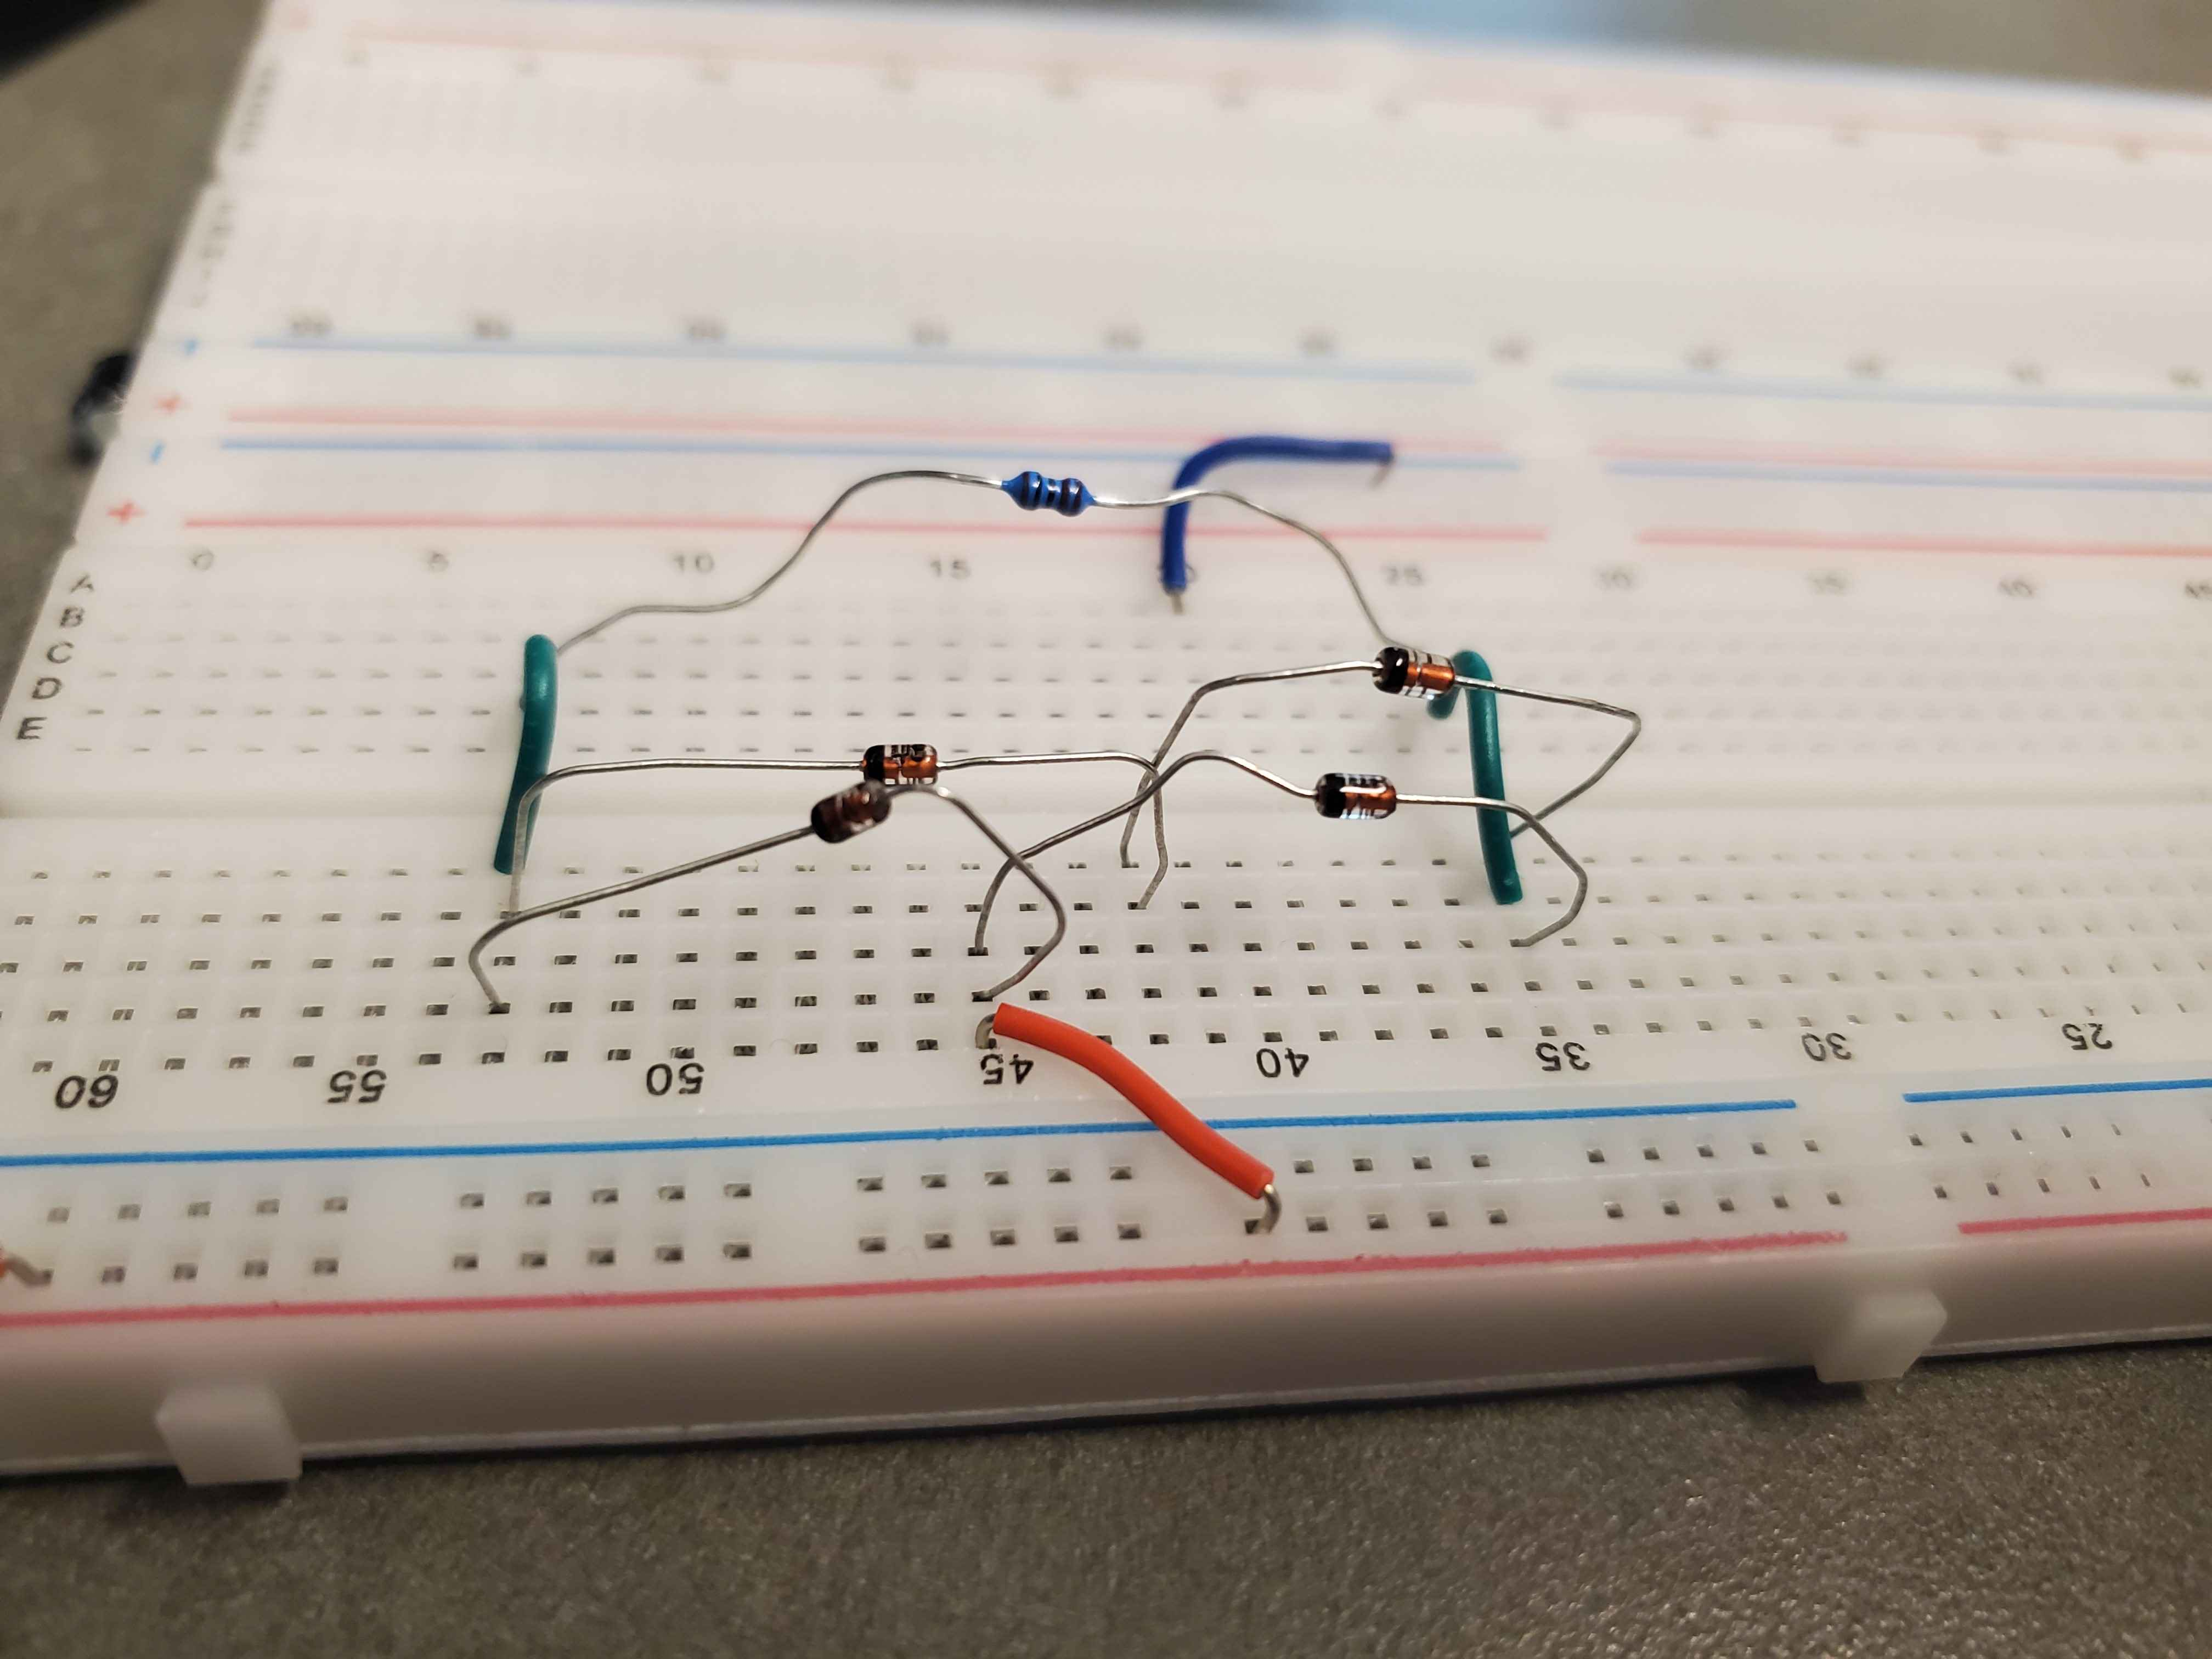
\includegraphics[width=9cm]{20240703_130140}}\hfil
		\subfloat[\centering LTSpice + Rudimentary Schematic Full-Wave Bridge Rectifier with output filter and Zener diode regulator as its output]{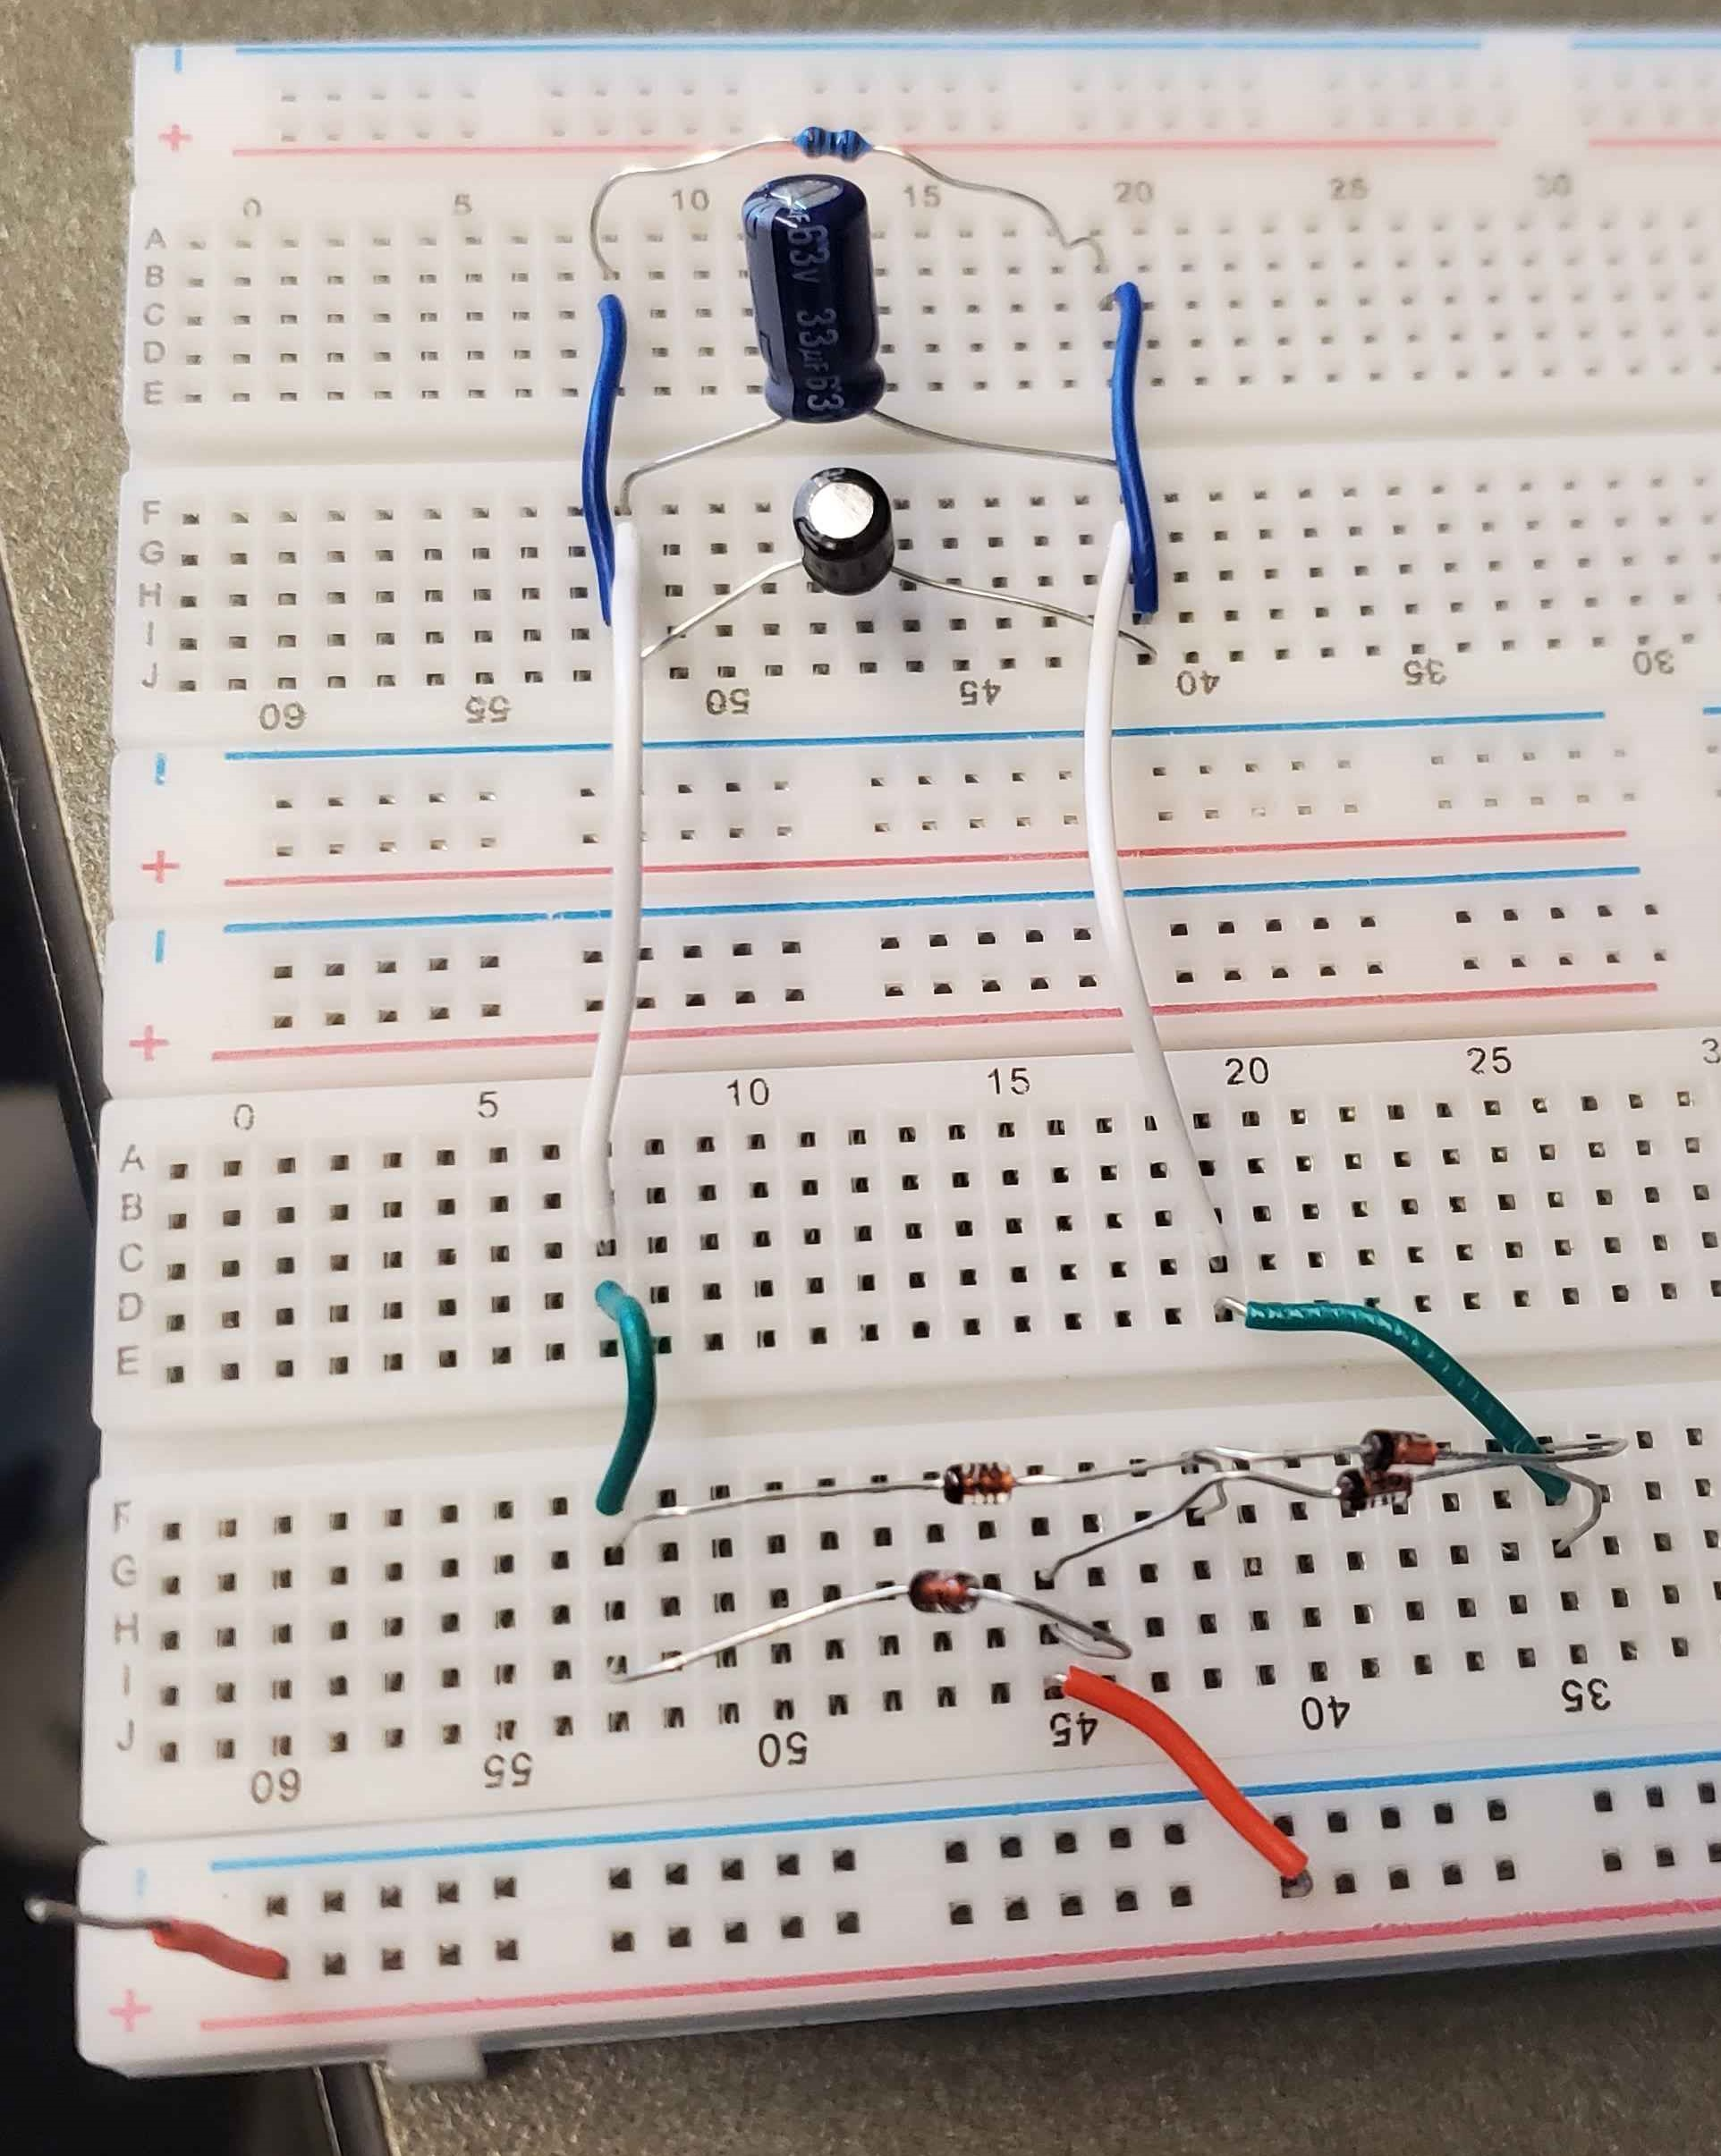
\includegraphics[width=6cm]{20240703_131410}}\hfil
	\end{figure}
	
	\nsection{Descriptions of Measurements \& Calculations}
	Given the default theoretical calculation for a Diode in forward-bias: $I_D=I_S(e^{\frac{V_D}{V_T}}-1)$; the dataset is similar in-nature - not exact because the characteristics of this diode differs - from section 1.1 of the lab.\\
	The characteristic of a \textit{Zener} Diode is its relationship to $-V_D$, as $I_D$ enters \textbf{Reverse-Breakdown} @ $-V_{Z0}$; the point of breakdown.\\
	The utilisation of the Capacitors in the Bridge Circuit is to dissipate the voltage curve over a gentler duration.
	Because of these characteristics, the Bridge Circuit essentially dampens and \emph{Rectifies} the entering voltage; $V_{in}$ to $V_o$
	\begin{figure}[h!]
		\centering
		\caption{Bridge Rectifier Circuits Scope}
		\subfloat[\centering Full-Wave Bridge Rectifier]{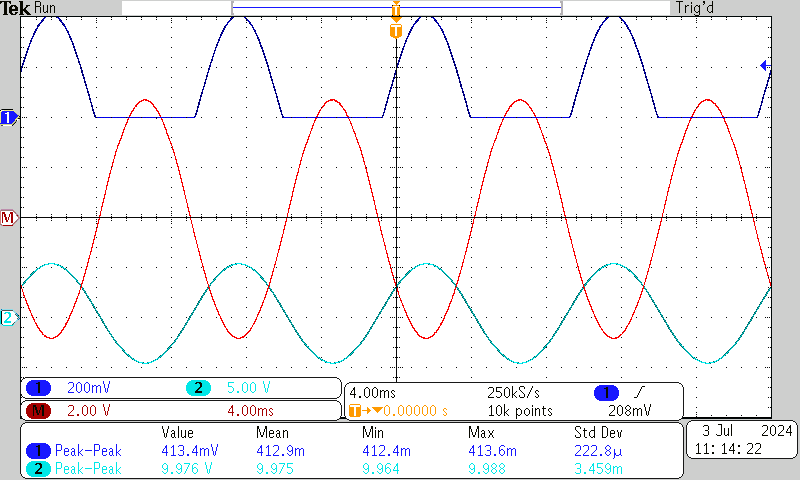
\includegraphics[width=9cm]{tek0000a}}\hfil
		\subfloat[\centering Full-Wave Bridge Rectifier with output filter]{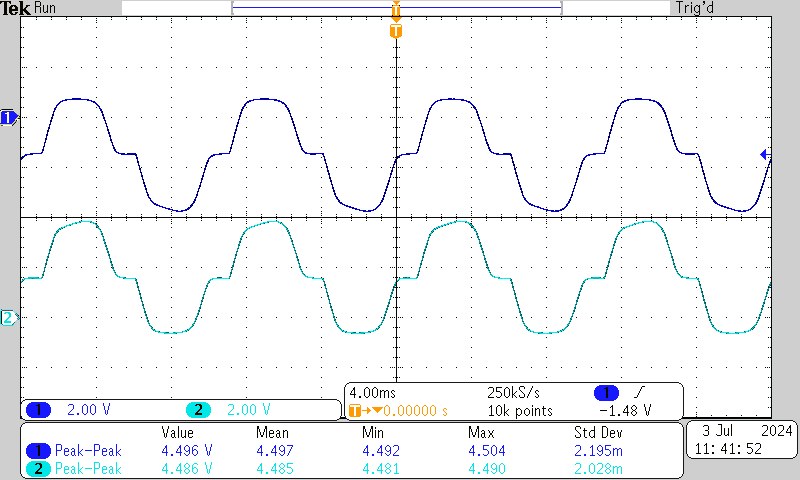
\includegraphics[width=9cm]{tek0001b}}\hfil
		\subfloat[\centering Full-Wave Bridge Rectifier with output filter and Zener diode regulator as its output]{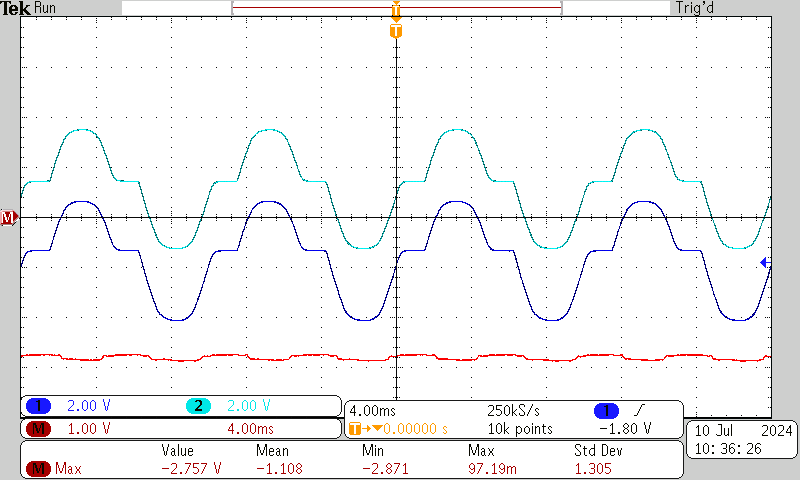
\includegraphics[width=9cm]{tek0001c}}
	\end{figure}
	
	\nsection{Summary \& Conclusions}
	Revealed in Figure RDD-Circuit 0A \& 0B, the generated oscilloscope readings of the two periodic function do in-fact dampen @ $V_{in}$ (CH2) greatly to $V_{out}$ (CH1). It is similary in the Series $D_Z$ circuit.
	\nsubsection{Discussion}
	\begin{itemize}
		\item \textbf{i. Compare the measured versus simulated data and explain any differences.}
		\subitem The measured and simulated data find differences in components, breakdown region, ideal components; which differs in threshold ranges and dampening ranges, and a consistent AC signal that has no attenuation.
		\item \textbf{ii. What are the purposes of experiment 1.41, 1.42, and 1.43? You can explain this by comparing the output voltage waveforms.}
		\subitem The purpose of 1.4.1 is to limit the negative values of the AC waveform. The output voltage had no voltage under 0.
		The purpose of 1.4.2 is to have the circuit charge the capacitors at the turn-on voltage for the diodes then when the input is low enough the capacitor will discharge slowly creating a more linear signal.
		\item \textbf{Is it desirable to reduce the output ripple voltage? Why do you think that is?}
		\subitem Signal alignment; although, we would have to consider using a secondary signal system to propgate the missing values - we'd have a consistently voltage running at a timer rate scaling with total Impedances and Voltage output.
		\subitem It could also be desirable to reduce the output voltage of the ripple because the output voltage might be used for other components that need a certain voltage to operate. So, the ripple voltage can be changed to meet those needs.
		\item \textbf{At what load resistance does the regulated full-wave bridge rectifier come out of regulation?}
		\subitem $R_{Load}\geq1k\Omega$
		\item \textbf{Explain how you would predict the minimum value of the load resistance for which the Zener diode still operates in the breakdown region.}
		\subitem Deriving the theoretical calculation of the Zener Diode's breakdown range; $V_o=V_i-R_i*_i$ @ $D_{Z_{BR}}$, and considering $R_{Load}\geq(R_2*\epsilon)$.
	\end{itemize}
	\newpage
	\newpage
	\nsection{Bibliography}
	\textbf{Cited:}\\
	\begin{itemize}
		\item Lab 1 Manual
		\item Sedra, Adel, and Kenneth Smith. Microelectronic Circuits. S.L., Oxford Univ Press Us, 2019.
		\item “How Do You Calculate, a Silicon Junction Diode with N = 1 Has v = 0.7 v al I = 1 MA. What Is the Voltage Drop at I=0.1 MA and I=10 MA.?” Quora, 2024, appliedmathematics.quora.com/How-to-calculate-A-silicon-junction-diode-with-n-1-has-v-0-7-V-al-I-1-mA-What-is-the-voltage-drop-at-I-0-1-mA-an?top\_ans=223007030. Accessed 15 July 2024.
	\end{itemize}
	\begin{figure}[!h]
		\subfloat[Look at her, she's perfect.]{
\includegraphics[width=\linewidth]{GodILoveFurina}}
	\end{figure}
\end{document}